\documentclass[tikz]{standalone}

\usepackage{newtxtext,newtxmath}

%!TEX root = main.tex

% mytikzset
\usepackage{tikz}
\usetikzlibrary{positioning,arrows,shapes,patterns}
\usetikzlibrary{decorations.pathmorphing}
\usetikzlibrary{decorations.markings}
\usetikzlibrary{decorations.pathreplacing}
\usetikzlibrary{calc}
\usetikzlibrary{patterns}
\usetikzlibrary{decorations.markings}
\usetikzlibrary{petri}

\tikzset{
  vector/.style={thick,double,draw=black, postaction={decorate},
    decoration={markings,mark=at position .6 with {\arrow[black,scale=0.4]{triangle 45}}}},
  axial/.style={thick,double,densely dashed,draw=black, postaction={decorate},
    decoration={markings,mark=at position .6 with {\arrow[black,scale=0.4]{triangle 45}}}},
  gluon/.style={decorate, draw=black,
    decoration={coil,aspect=0.3,segment length=5pt,amplitude=3pt}},
  pseudo/.style={thick, dashed, draw=black, postaction={decorate},
    decoration={markings,mark=at position .6 with {\arrow[red,scale=0.5]{triangle 45}}}},
  scalar/.style={thick,draw=black, postaction={decorate},
    decoration={markings,mark=at position .6 with {\arrow[black,scale=0.5]{triangle 45}}}},
  cut/.style={draw=black, decorate, decoration={snake, segment length=1mm, amplitude=0.2mm}}
}

\usetikzlibrary{decorations.pathreplacing}

\begin{document}
\nopagecolor
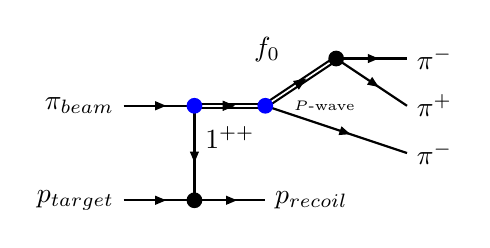
\begin{tikzpicture}[node distance=0.6cm and 0.9cm]
  \coordinate[label=left:$p_{\text{target}}$] (a1);
  \coordinate[    right=of a1] (a2);
  \coordinate[right=of a2,label=right:$p_{\text{recoil}}$] (a3);
  \coordinate[above=of a2] (z2);
  \coordinate[above=of z2] (b12);
  \coordinate[left=of b12,label=left:$\pi_{\text{beam}}$] (b1);

  \coordinate[right=of b12,label=right:{\tiny \quad $P$-wave}] (b2);
  \coordinate[above right=of b2] (b13);
  \coordinate[below right=of b13,label=right:$\pi^+$] (b3);
  \coordinate[right=of b13,label=right:$\pi^-$] (b4);
  \coordinate[right=of b2] (b25);
  \coordinate[below right=of b25,label=right:$\pi^-$] (b5);

  \draw[scalar]  (a1) -- (a2);
  \draw[scalar]  (a2) -- (a3);
  \draw[scalar]  (b12) -- (a2);
  \draw[scalar]  (b1) -- (b12);
  \draw[vector]  (b12) -- node[label=below:{$1^{++}$}] {} (b2);
  \draw[scalar]  (b13) -- (b3);
  \draw[vector]  (b2) -- node[label=above left:{$f_0$}] {} (b13);
  \draw[scalar]  (b2) -- (b5);
  \draw[scalar]  (b13) -- (b4);

  \fill[blue]  (b2) circle [radius=0.1];
  \fill[blue] (b12) circle [radius=0.1];
  \fill[black] (a2) circle [radius=0.1];
  \fill[black] (b13) circle [radius=0.1];
\end{tikzpicture}
\end{document}
